\documentclass[article]{jss}
\usepackage[utf8]{inputenc}

\providecommand{\tightlist}{%
  \setlength{\itemsep}{0pt}\setlength{\parskip}{0pt}}

\author{
Alwin Wang\\Monash University
}
\title{Visualising Serve Trajectories in High-Performance Tennis with R}
\Keywords{keywords, not capitalized, \proglang{Java}, REMEMBER TO ADD TITLES TO YOUR GRAPHS}

\Abstract{
This paper investigates methods to effectively visualise key
characteristics of serves using trajectory of elite tennis athletes
provided by Tennis Australia. The key characteristics identified were
the position, velocity and spin of a ball as well as the location of
single and multiple serve clusters. For the visuals presented in the
paper, a sample of 2000 serves from the 2016 Australian Open from thirty
three servers was used.
}

\Plainauthor{Alwin Wang}
\Plaintitle{Visualising Serve Trajectories in High-Performance Tennis with R}
\Shorttitle{Visualising Serves}
\Plainkeywords{keywords, not capitalized, Java, REMEMBER TO ADD TITLES TO YOUR GRAPHS}

%% publication information
%% \Volume{50}
%% \Issue{9}
%% \Month{June}
%% \Year{2012}
\Submitdate{}
%% \Acceptdate{2012-06-04}

\Address{
    Alwin Wang\\
  Monash University\\
  First line Second line\\
  E-mail: \href{mailto:awan39@student.monash.edu}{\nolinkurl{awan39@student.monash.edu}}\\
  URL: \url{http://rstudio.com}\\~\\
  }

\usepackage{amsmath}

\begin{document}

\section{Introduction}\label{introduction}

This template demonstrates some of the basic latex you'll need to know
to create a JSS article.

\section{Shape}\label{shape}

\subsection{Position}\label{position}

asdfaslkfj asfldkjasd f

\begin{CodeChunk}
\begin{figure}

{\centering 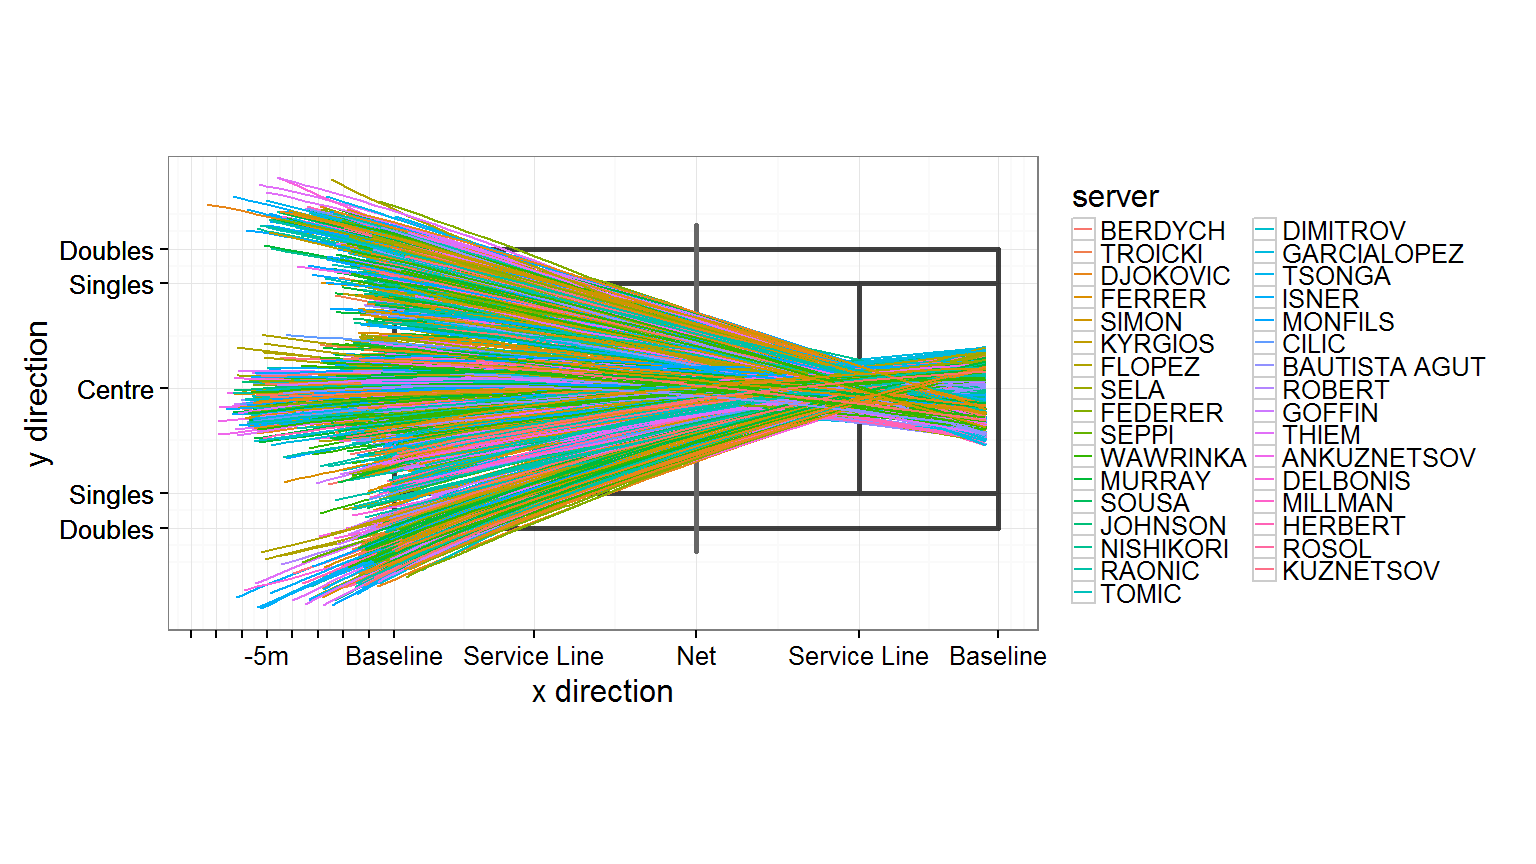
\includegraphics{vis-serve-article_files/figure-latex/all_topdown-1} 

}

\caption[All serves as overlayed lines]{All serves as overlayed lines}\label{fig:all_topdown}
\end{figure}
\end{CodeChunk}

\begin{CodeChunk}
\begin{figure}

{\centering \includegraphics{vis-serve-article_files/figure-latex/all_topdown_hexbin-1} 

}

\caption[Frequency of serves in hexagonal bins]{Frequency of serves in hexagonal bins}\label{fig:all_topdown_hexbin}
\end{figure}
\end{CodeChunk}

\begin{CodeChunk}
\begin{figure}

{\centering \includegraphics{vis-serve-article_files/figure-latex/all_topdown_height-1} 

}

\caption[Average height of serves in hexagonal bins]{Average height of serves in hexagonal bins}\label{fig:all_topdown_height}
\end{figure}
\end{CodeChunk}

\begin{CodeChunk}
\begin{figure}

{\centering \includegraphics{vis-serve-article_files/figure-latex/all_topdown_speed-1} 

}

\caption[Average impact speed in hexagonal bins]{Average impact speed in hexagonal bins}\label{fig:all_topdown_speed}
\end{figure}
\end{CodeChunk}

\begin{CodeChunk}
\begin{figure}

{\centering \includegraphics{vis-serve-article_files/figure-latex/all_topdown_vel-1} 

}

\caption[Average true velocity in hexagonal bins]{Average true velocity in hexagonal bins}\label{fig:all_topdown_vel}
\end{figure}
\end{CodeChunk}

\begin{CodeChunk}
\begin{figure}

{\centering \includegraphics{vis-serve-article_files/figure-latex/all_topdown_side-1} 

}

\caption[Scorer in hexagonal bins]{Scorer in hexagonal bins}\label{fig:all_topdown_side}
\end{figure}
\end{CodeChunk}

\begin{CodeChunk}
\begin{figure}

{\centering \includegraphics{vis-serve-article_files/figure-latex/all_topdown_classname-1} 

}

\caption[Serve type in hexagonal bins]{Serve type in hexagonal bins}\label{fig:all_topdown_classname}
\end{figure}
\end{CodeChunk}

\begin{CodeChunk}
\begin{figure}

{\centering \includegraphics{vis-serve-article_files/figure-latex/all_topdown_hextriclass-1} 

}

\caption[Serve type using Hextri]{Serve type using Hextri}\label{fig:all_topdown_hextriclass}
\end{figure}
\end{CodeChunk}

\subsection{Landing}\label{landing}

\begin{CodeChunk}
\begin{figure}

{\centering \includegraphics{vis-serve-article_files/figure-latex/all_topdown_landsplitscorer-1} 

}

\caption[Split landing position coloured by scorer]{Split landing position coloured by scorer}\label{fig:all_topdown_landsplitscorer}
\end{figure}
\end{CodeChunk}

\begin{CodeChunk}
\begin{figure}

{\centering \includegraphics{vis-serve-article_files/figure-latex/all_topdown_landsplitnum-1} 

}

\caption[Split landing position coloured by serve number]{Split landing position coloured by serve number}\label{fig:all_topdown_landsplitnum}
\end{figure}
\end{CodeChunk}

\begin{CodeChunk}
\begin{CodeInput}
R> plot_gg <- plot_perserve %>% filter(serve_classname != "Fault")
R> court_service + 
R+     geom_density2d(data = plot_gg, aes(x=center.x, y=center.y)) #+ 
\end{CodeInput}
\begin{figure}

{\centering \includegraphics{vis-serve-article_files/figure-latex/all_landingcontoursguass-1} 

}

\caption[Countour plot of all serves using ]{Countour plot of all serves using }\label{fig:all_landingcontoursguass}
\end{figure}
\begin{CodeInput}
R>   # facet_grid(side~serve_classname)
\end{CodeInput}
\end{CodeChunk}

\textbackslash{}begin\{CodeChunk\} \textbackslash{}begin\{CodeInput\}
R\textgreater{} factor1 \textless{}-
as.data.frame(levels(plot\_perserve\$side)) R\textgreater{} factor2
\textless{}- MultipleGames(4,perserve = TRUE, server = TRUE)
\textbackslash{}end\{CodeInput\} \textbackslash{}end\{CodeChunk\}

\begin{CodeChunk}
\begin{CodeInput}
R> plot_Ad <- plot_perserve %>% filter(side == "Ad")
R> densAd <- kde2d(plot_Ad$center.x, plot_Ad$center.y, 
R+               lims = c(-6.4, 0, 0, 4.115))
R> plot_Ad <- data.frame(expand.grid(center.x = densAd$x, center.y = densAd$y),
R+                      z = as.vector(densAd$z))
R> plot_Du <- plot_perserve %>% filter(side == "Deuce")
R> densDu <- kde2d(plot_Du$center.x, plot_Du$center.y, 
R+               lims = c(-6.4, 0, -4.115, 0))
R> plot_Du <- data.frame(expand.grid(center.x = densDu$x, center.y = densDu$y),
R+                      z = as.vector(densDu$z))
R> court_service + 
R+   geom_contour(aes(x=center.x, y=center.y,z=z), data = plot_Ad) +
R+   geom_contour(aes(x=center.x, y=center.y,z=z), data = plot_Du) #+ 
\end{CodeInput}
\begin{figure}

{\centering \includegraphics{vis-serve-article_files/figure-latex/all_landingcontourslimits-1} 

}

\caption[Countour plot of all serves using ]{Countour plot of all serves using }\label{fig:all_landingcontourslimits}
\end{figure}
\begin{CodeInput}
R>   # facet_grid(side~serve_classname)
\end{CodeInput}
\end{CodeChunk}

\url{http://stackoverflow.com/questions/12394321/r-what-algorithm-does-geom-density-use-and-how-to-extract-points-equation-of}

\begin{CodeChunk}
\begin{figure}

{\centering \includegraphics{vis-serve-article_files/figure-latex/landing_contours4games-1} 

}

\caption[To Fixx]{To Fixx}\label{fig:landing_contours4games}
\end{figure}
\end{CodeChunk}

\section{Spin}\label{spin}

\begin{CodeChunk}
\begin{figure}

{\centering \includegraphics{vis-serve-article_files/figure-latex/coolarc_behind-1} 

}

\caption[Example of the effect of spin]{Example of the effect of spin}\label{fig:coolarc_behind}
\end{figure}
\end{CodeChunk}

\subsection{Code formatting}\label{code-formatting}

Don't use markdown, instead use the more precise latex commands:

\begin{itemize}
\tightlist
\item
  \proglang{Java}
\item
  \pkg{plyr}
\item
  \code{print("abc")}
\end{itemize}

\section{R code}\label{r-code}

Can be inserted in regular R markdown blocks.

\begin{CodeChunk}
\begin{CodeInput}
R> x <- 1:10
R> x
\end{CodeInput}
\begin{CodeOutput}
 [1]  1  2  3  4  5  6  7  8  9 10
\end{CodeOutput}
\end{CodeChunk}



\end{document}

